\documentclass{article}

% The file ijcai16.sty is the style file for IJCAI-16 (same as ijcai07.sty).
\usepackage{ijcai16}

% Use the postscript times font!
\usepackage{times}

% the following package is optional:
%\usepackage{latexsym} 

\usepackage[utf8]{inputenc}
\usepackage{amsmath}
\usepackage{amsfonts}
\usepackage{graphicx}
\usepackage{subfig}  
\usepackage{url}

\graphicspath{{figs/}}

% Following comment is from ijcai97-submit.tex:
% The preparation of these files was supported by Schlumberger Palo Alto
% Research, AT\&T Bell Laboratories, and Morgan Kaufmann Publishers.
% Shirley Jowell, of Morgan Kaufmann Publishers, and Peter F.
% Patel-Schneider, of AT\&T Bell Laboratories collaborated on their
% preparation.

% These instructions can be modified and used in other conferences as long
% as credit to the authors and supporting agencies is retained, this notice
% is not changed, and further modification or reuse is not restricted.
% Neither Shirley Jowell nor Peter F. Patel-Schneider can be listed as
% contacts for providing assistance without their prior permission.

% To use for other conferences, change references to files and the
% conference appropriate and use other authors, contacts, publishers, and
% organizations.
% Also change the deadline and address for returning papers and the length and
% page charge instructions.
% Put where the files are available in the appropriate places.

\title{A Space CoBot for personal assistance in space stations\thanks{This work was
supported by the FCT project [UID/EEA/50009/2013].}}
\author{Pedro Roque \qquad Rodrigo Ventura \\
  Institute for Systems and Robotics \\
  Instituto Superior Técnico, Universidade de Lisboa \\
  Av. Rovisco Pais, 1, 1049-001 Lisboa, Portugal \\
  pedro.roque@tecnico.ulisboa.pt, rodrigo.ventura@isr.tecnico.ulisboa.pt}

\begin{document}

\maketitle

\begin{abstract}
  Microgravity environments inside inhabited space stations are
  particularly challenging for service robots, being quite different
  from Earth in various ways. In this paper we propose
  and discuss the design and applicability of a collaborative aerial
  robot, called Space CoBot, to provide personal assistance to
  astronauts in microgravity environments. The platform is based on a
  modular holonomic aerial vehicle with an hexarotor configuration. In
  this paper we explore the feasibility of using Space CoBot for
  performing two tasks: (1) scavenging afloat waste and
  (2) stabilization of astronaut motion.  Scavenging is performed by
  tracking and sucking debits, while stabilization aims at
  driving to zero the motion of an astronaut attached to the robot. A
  convergent motion controller is used for guidance of the vehicle to
  accomplish both tasks. We provide simulation results on a realistic
  simulator to illustrate the feasibility of the approach.
\end{abstract}


\section{Introduction}
\label{sec:introduction}

Transporting to and maintaining astronauts in orbiting space stations is
hard: space flight is risky and the costs associated with life
maintenance are extremely high. Thus, it is desirable that crew sizes
are kept small. In this context, the use of
autonomous service robots that perform collaborative tasks with humans
(CoBots) is particularly interesting.

In this paper we explore the design and the application of a robot, called
Space CoBot, for collaborative tasks with astronauts in the interior
of a space station. 
This is a microgravity environments with
breathable air at atmospheric pressure, thus allowing propeller based
propulsion. Space CoBot exploits these properties being an aerial
vehicle based on a hexarotor design. This design allows for a fully
omnidirectional (holonomic) motion (6 Degrees of Freedom - 6-DoF),
while being based in electrical motors and propellers is mechanically
simple and reliable.

We envision a broad range of services Space CoBot may provide to
astronauts.
One broad class is telepresence, improving
collaboration among the onboard and Earth crews. In particular, Space
CoBot may be used to provide an immersive experience of the Earth
crew, as well as enabling face-to-face communication with astronauts.
Another broad class is small object management, that
is, tracking and manipulating small free flying objects, such as pens,
screws, pins, etc. This has been identified as a challenge specific to
microgravity environments (\cite{stuster86}, page~105). In this paper
we address this latter class, providing two example applications:
(1)~debris scavenging, that is, the problem of catching disposing of small free
flying objects, and (2)~astronaut body stabilization, that is,
preventing their body to drift afloat while working.

The idea of aerial vehicles inside space stations is not new. The NASA
project SPHERES (Synchronized Position Hold Engage Reorient
Experimental Satellites) started in 2000 with the design of a small
pressurized air propulsion vehicle~\cite{miller00}. In 2006 three
SPHERES units were deployed aboard the International Space Station
(ISS)~\cite{nolet07}. More recently, NASA proposed the Astrobee
vehicle, with a simpler propulsion system based on several centrifugal
fans and nozzles~\cite{bualat15}. The Astrobee also features a 2-DoF
arm and docking capability.

Omnidirectional multirotors have been proposed in the past, but the
literature is scarce. In~\cite{jiang13,voyles12} a dexterous
hexarotor has been proposed, where the holonomic kinematics is
used for dexterous manipulation. More recently, the design and control
of an eight-rotor aerial vehicle has been proposed
in~\cite{bescianini16}, featuring a design optimization approach very
similar to ours.

This paper is structured as follows: sections~\ref{sec:vehicle-design}
and~\ref{sec:posit-attit-contr} describe the design of Space CoBot and
the proposed motion controller, summarizing~\cite{yoda:arxiv16a},
sections~\ref{sec:debis-scavenging} and~\ref{sec:astr-stab} describe
our approach to the debris scavenging and astronaut stabilization
tasks, simulation results are presented in
section~\ref{sec:sim-res}, and section~\ref{sec:concl-future-work}
wraps up the paper with some conclusions and future work.


\section{Vehicle Design}
\label{sec:vehicle-design}

\begin{figure*}
  \def\gscale{0.28}
  \centering
  \subfloat[]{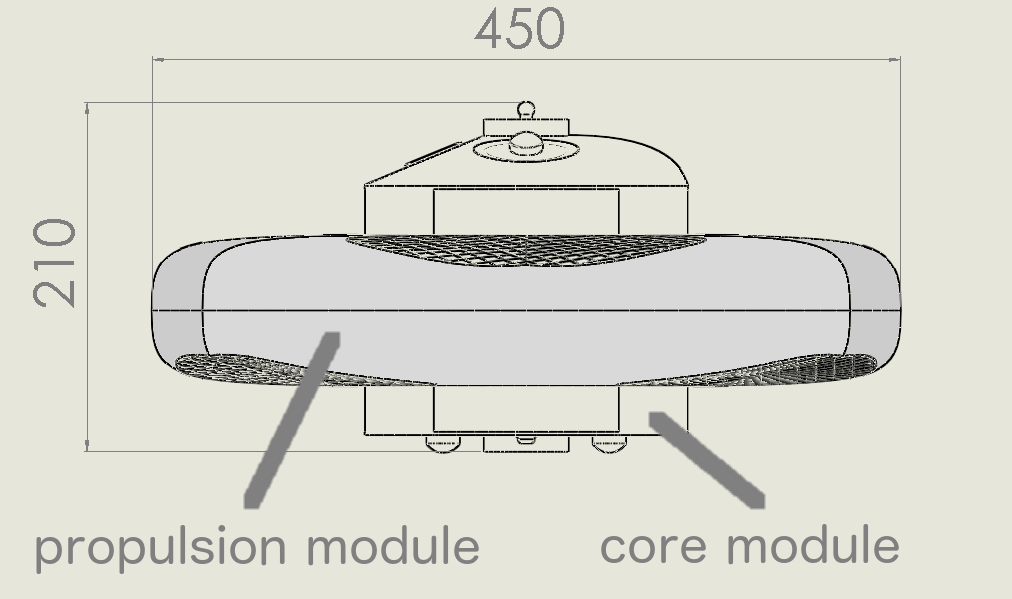
\includegraphics[height=\gscale\linewidth]{figs/side_view.png}}
  \hfil
  \subfloat[]{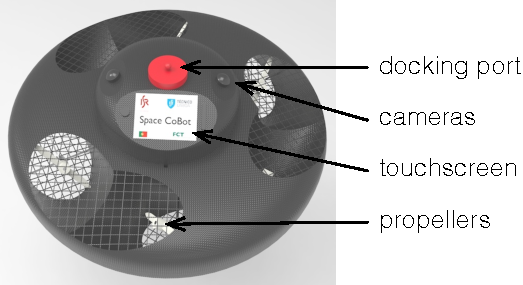
\includegraphics[height=\gscale\linewidth]{figs/per_render_labeled.pdf}}
  \caption{Design of the Space CoBot: (a)~side view
  with the core and propulsion modules indicated with dimensions in
  millimeters; (b)~CAD rendering showing some of the main components.}
  \label{fig:modules}
\end{figure*}

The design of Space CoBot is modular, comprising an outer propulsion
module and an inner core module, illustrated in
Figure~\ref{fig:modules}. The propulsion module comprises six
propellers, arranged in such a way the motion is fully holonomic. We
further detail this module below. The core module contains the power
supply (battery), interface electronics, computers, a touchscreen, an
array of video cameras for perception and telepresence, and an
inertial measurement unit (IMU). This module can be easily extended
with other components, such as a robotic arm.
The user interface can either be based on the onboard touchscreen or
on a remote device, such as a tablet or a wearable device. Current multitouch technology is
very sensitive to touch, so we expect the touch pressure to be
negligible when compared with the weight of the robot and its
capability of using its
propulsion system to compensate any motion provoked by the touching.
We consider vision-based navigation,
using the camera array. At the opposite sides of the core module we
include two docking ports, for two purposes: (1) charging the
batteries and (2) attachment to another Space CoBot (see
Figure~\ref{fig:docking}). The design of these docking ports follows previous
work described in~\cite{yoda:raposa:industrial}.

\begin{figure}
  \centering
  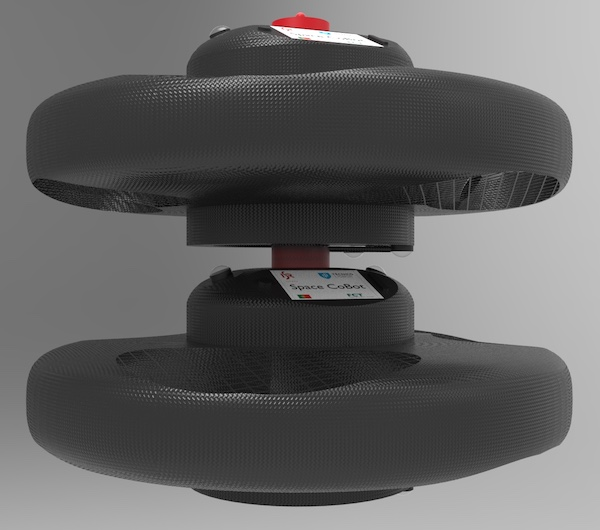
\includegraphics[width=0.8\linewidth]{figs/side_render.jpg}
  \caption{Render of two Space CoBots rigidly attached through their docking
    ports.}
  \label{fig:docking}
\end{figure}

\begin{figure}
  \centering
  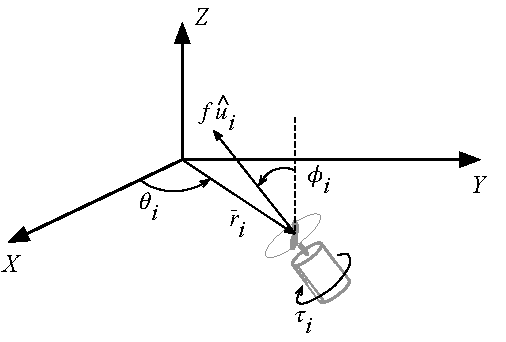
\includegraphics[width=0.8\linewidth]{prop.pdf}
  \caption{Notation used for modeling a single propeller with respect
    to the body frame of the robot, centered on its center of mass.}
  \label{fig:prop}
\end{figure}

The propulsion module is based on a hexarotor design, where the
rotation axes of the six propellers are not parallel. Rather, each
propeller $i=1,\ldots,6$ has an angular offset $\phi_i$ from the $Z$ axis, as shown in
Figure~\ref{fig:prop}. Each such propeller contributes with a force
$\bar{F}_i$ and a torque $\bar{M}_i$ on the robot center of mass (CoM), given by the following
expression~\cite{yoda:arxiv16a}, following the notation of this figure:
\begin{equation}
  \begin{aligned}
    &\left(
      \begin{array}{c}
        \bar{F}_i \\
        \bar{M}_i
      \end{array}
    \right) = \bar{a}_i\,u_i \\
    &\bar{a}_i = \left(
      \begin{array}{c}
        K_1 \hat{u}_i \\
        K_1 \bar{r}_i \times \hat{u}_i - w_i K_2 \hat{u}_i
      \end{array}\right)
  \end{aligned}
\end{equation}
where $\times$ denotes vector cross product, $u_i$ is the actuation
signal, and $w_i$ is a flag with value either $-1$ or $1$ depending on
whether the propeller rotates clockwise or anti-clockwise for a
positive thrust long $\hat{u}_i$.  Constants $K_1$ and $K_2$ are given by
\begin{equation}
  \label{eq:blade}
  K_1 = \rho D^4 C_T \qquad K_2 = \frac{\rho D^5}{2\pi} C_P
\end{equation}
where $\rho$ is the air density, $D$ is the propeller diameter, and
the $C_T$ and $C_P$ are blade dependent dimensionless constants called
thrust and power coefficients, following the momentum-blade element
theory~\cite{mccormick95}. The actuation signal is $u_i=n_i^2$, where
$n_i$ is the blade revolutions per second of propeller~$i$. We will
adopt $u_i$ as the input signal for the $i$-th motor controller, to
maintain a linear relation between actuation and forces/torques.

Since the contributions of each propeller is expressed in the same
reference frame, the net force and torque will be given by the sum of
these contributions. This sum can be put in matrix form as
\begin{equation}
  \label{eq:au}
  \left(
    \begin{array}{c}
      \bar{F} \\
      \bar{M}
    \end{array}
  \right) = \mathbf{A}\,\bar{u}
\end{equation}
where $\mathbf{A}=[\bar{a}_1 \cdots \bar{a}_N]$ is a square matrix,
hereby called \emph{actuation matrix}, and $\bar{u}=[u_1\cdots u_N]^T$
is the actuation input vector. The crucial observation is that, if the
actuation matrix $\mathbf{A}$ is at least rank 6, the linear
equation~\eqref{eq:au} can be solved for $\bar{u}$ for any given
combination of $\bar{F}$ and $\bar{M}$.  A necessary (but not
sufficient\footnote{Sufficiency requires $\mathbf{A}$ to be full
  rank.}) condition for this to be true is to have at least 6
propellers, thus justifying the hexarotor design. Note that this
matrix only depends on these parameters: angles $\{\theta_i\}$ and
$\{\phi_i\}$, distance $d$, the trust coefficients $K_1$, $K_2$, and
$\{w_i\}$.

As mentioned before, if the axes of all propellers were parallel,
$\{\phi_i=0\}$, holonomy would be lost. The question is then which angle values to
choose. Considering that the thrust is
bounded, the value of these angles hold a direct relationship with the
maximum force and torque attainable along an arbitrary direction. For
instance, when all propeller axes are parallel, one gets maximum
thrust along the $Z$ axis, but zero along any orthogonal direction; as
these angles depart from zero, we are able to tradeoff the maximum
thrust along $Z$ with non-zero maximum thrust along any given orthogonal
directions. In~\cite{yoda:arxiv16a} we addressed this problem by formulating
it as a multi-criteria optimization problem. We summarize the main
results below.

We consider each actuation signal to be
bounded between $-1$ and $1$, that is,
\begin{equation}
  \label{eq:ahcube}
  -1 \leq u_i \leq 1 \quad \text{for} \quad i=1,\ldots,6
\end{equation}
since~\eqref{eq:au} is linear, and thus the optimization problem is
invariant to the scaling of these signals.  According to
\eqref{eq:au}, this hypercube will map onto a 6-dimensional convex
polyhedron\footnote{A convex polyhedron is an intersection of a finite
  number of half-spaces.} in the $(\bar{F}, \bar{M})$
space. Our goal will be to find the configurations of angles
$\{\phi_i\}$ and flags $\{w_i\}$ that maximize the range
of forces (and torques) over all directions.  Geometrically, this
corresponds to changing $\{\phi_i\}$ and $\{w_i\}$ such that a ball of
nonzero radius can fit inside the 3-dimensional convex polyhedron in
the $\bar{F}$ space mapped by the actuation hypercube
in~\eqref{eq:ahcube}, while keeping zero torque, $\bar{M}=0$. A
similar reasoning applies to the torque space $\bar{M}$, while keeping
$\bar{F}=0$.

Since we intend to both maximize force and torque, we make the
trade-off between the two explicit by taking a multi-criteria
optimization approach. The formulation of this problem is detailed
in~\cite{yoda:arxiv16a}, having the following form:
\begin{equation}
  \label{eq:multi}
  \begin{aligned}
    &\text{minimize}\:(p, q) \\
    &\text{subject to:} \\
    &\quad p \geq \|b_i\|^2, i=1,\ldots,6 \\
    &\quad q \geq \|c_i\|^2, i=1,\ldots,6
  \end{aligned}
\end{equation}
In this problem, the optimization variables are
$\{p,q\}\cup\{\phi_i\}\cup\{w_i\}$ and the cost functions are $p$ and
$q$. For the sake of symmetry we kept the angles~$\{\theta_i\}$
equally spaced in $60$ deg intervals. Intuitively, $p^{-1}$ and
$q^{-1}$ correspond to the radius of the above mentioned balls in the $\bar{F}$ and
$\bar{M}$ spaces, respectively. Minimizing $p$ or $q$, subject to the
problem constraints, correspond to
maximizing the radius of the balls that fit inside the polyhedrons
mapped by the bounded actuation.

The solution of this
multi-criteria optimization problem is the set $\mathcal{P}$ of
non-dominated solutions, also known as the \emph{Pareto optimal
  set}~\cite{statnikov95}. We obtained a numerical approximation to
this set, from which we chose a solution maximizing the force
component, since the corresponding maximum torque is not significantly
lower than other non-dominated solutions~\cite{yoda:arxiv16a}. This
solution\footnote{The angles are rounded off to the nearest degree
  unit for the sake of simplicity. However, the impact of this on the
  cost is minimal.} is shown in Table~\ref{tab:selected}. All of the following
results shown in this paper use this selected configuration.

\begin{table}
  \centering
  \begin{tabular}{ccccccc}
    propeller ($i$) & 1 & 2 & 3 & 4 & 5 & 6 \\
    \hline
    $\theta_i$ & 0 & 60 & 120 & 180 & 240 & 300 \\
    $\phi_i$ & 55 & -55 & 55 & -55 & 55 & -55 \\
    $w_i$ & -1 & 1 & -1 & 1 & -1 & 1 \\
    \hline
  \end{tabular}
  \caption{Design parameters of the selected solution. Both
    $\{\theta_i\}$ and $\{\phi_i\}$ are expressed in degrees.}
  \label{tab:selected}
\end{table}


\section{Position and Attitude Control}
\label{sec:posit-attit-contr}

The dynamical model of the vehicle can be
derived from the Newton and Euler equations of motion. Let us denote the position and velocity of the
body frame $\mathcal{B}$, centered on the vehicle CoM and aligned
according to Figure~\ref{fig:prop}, with respect to the inertial frame
$\mathcal{I}$ as $\bar{x}$ and $\bar{v}$, the rotation matrix of frame
$\mathcal{B}$ with respect to $\mathcal{I}$ as $\mathbf{R}$, and the
angular velocity of the vehicle in the body frame $\mathcal{B}$ as
$\bar{\omega}$. Then,
\begin{equation}
  \label{eq:dynsys}
  \left\{
    \begin{aligned}
      \dot{\bar{x}} &= \bar{v} \\
      m \dot{\bar{v}} &= \mathbf{R} \bar{F} \\
      \dot{\mathbf{R}} &= \mathbf{R}\,\mathbf{S}(\bar{\omega}) \\
      \mathbf{J} \dot{\bar{\omega}} &= \bar{M} - \bar{\omega}\times\mathbf{J} \bar{\omega}
    \end{aligned}
  \right.
\end{equation}
where the constants $m$ and $\mathbf{J}$
are the vehicle's mass and moment of inertia, while
$\mathbf{S}(\bar{\omega})$ is the skew-symmetric matrix defined by
\begin{equation}
  \label{eq:S}
  \mathbf{S}(\bar{\omega}) =
  \left[
    \begin{array}{ccc}
      0 & -\omega_z & \omega_y \\
      \omega_z & 0 & -\omega_x \\
      -\omega_y & \omega_x & 0 \\
    \end{array}
  \right]
\end{equation}
for $\bar{\omega}=[\omega_x\:\omega_y\:\omega_z]^T$. Note the absence
of the gravity force in this model.

The approach used for the motion control of the vehicle exploits its
holonomic design by
decoupling the translational and rotational modes. To do so, we first
apply feedback linearization~\cite{sastry99} to the translational part
of~\eqref{eq:dynsys}:
\begin{equation}
  \label{eq:fctrl}
    \left\{
    \begin{aligned}
      \dot{\bar{x}} &= \bar{v} \\
      \dot{\bar{v}} &= \bar{p} \\
      \bar{F} &= m \mathbf{R}^T \bar{p}
    \end{aligned}
  \right.
\end{equation}
and then design a feedback controller for $\bar{p}$. Since this
dynamical system is diagonal and second order, a PD controller is
enough to ensure exponential
convergence:
\begin{equation}
  \label{eq:pctrl}
  \begin{aligned}
    \bar{e}_x &= \bar{x} - \bar{x}_d \\
    \bar{e}_v &= \bar{v} - \bar{v}_d \\
    \bar{p} &= -k_x \bar{e}_x -k_v \bar{e}_v \\
  \end{aligned}
\end{equation}
where $\bar{x}_d$ and $\bar{v}_d$ are the desired position and
velocity vectors in the inertial frame~$\mathcal{I}$, and $k_x$ and
$k_v$ are the proportional and derivative gains of the PD controller.

For the attitude control we follow the exponentially convergent $SO(3)$ controller
proposed in~\cite{lee12}:
\begin{equation}
  \label{eq:mctrl}
  \begin{aligned}
    \bar{e}_R &= \frac{1}{2 \sqrt{1+tr[\mathbf{R}^T_d\mathbf{R}]} } S^{-1}( \mathbf{R}^T_d \mathbf{R} -
    \mathbf{R}^T \mathbf{R}_d ) \\
    \bar{e}_\omega &= \bar{\omega} - \mathbf{R}^T
    \mathbf{R}_d\,\bar{\omega}_d \\
    \bar{M} &= -k_R\,\bar{e}_R - k_\omega\,\bar{e}_\omega \\
    &+S^{-1}(\mathbf{R}^T\mathbf{R}_d\bar{\omega}_d)\mathbf{J}\mathbf{R}^T\mathbf{R}_d\bar{\omega}_d 
    +\mathbf{J}\mathbf{R}^T\mathbf{R}_d\dot{\bar{\omega}}_d \\
  \end{aligned}
\end{equation}
where $\mathbf{R}_d$ is the rotation matrix of the desired attitude,
$\bar{\omega}_d$ is the desired angular velocity vector, with $k_R$ and
$k_\omega$ as controller gains. The $S^{-1}$ function performs the inverse
operation as the one defined in~\eqref{eq:S}, that is, recovers
the vector from a given skew-symmetric matrix.

\begin{figure}
  \centering
  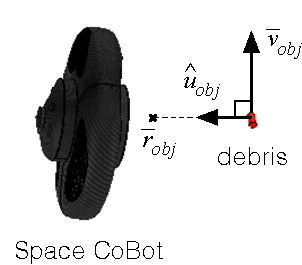
\includegraphics[width=0.6\linewidth]{figs/debris_geometry.pdf}
  \caption{Geometry of the debris scavenging problem.}
  \label{fig:debris_geom}
\end{figure}

\section{Debris Scavenging}
\label{sec:debis-scavenging}

One distinctive feature of microgravity environments is that objects
do not fall down to the floor when unreleased from one's hand. In a space
station environment, unattached objects, such as food debris, pens,
and even liquids, fly freely until coliding with something else, e.g.,
a wall. Therefore, astronats are required to manage manually such
objects, demanding additional cognitive effort~\cite{stuster86}.
We propose here the automatic management of these objects by
Space CoBot. That is, we consider this robot to be able to detect and
track free flying debris, e.g., by the use of its camera array, and to
be equipped with a small vacuum cleaner capable of capturing and
storing them internally.

To provide a proof of concept for this task, we considered a small
object flying freely in an uncluttered environment. Since it
is free, the linear and angular velocities are constant. To
capture it we consider a three phase process: first, the Space CoBot
matches its trajectory at a distance $D_1$ of the object;
second, it approaches the object at a constant velocity with respect
to it until a threshold distance $D_2$ is achieved, where we consider it to be within reach of a small onboard vacuum
cleaner; finally, the object 
is sucked into the vehicle by it.

The geometry of the problem is shown in
Figure~\ref{fig:debris_geom}.
Let $\bar{x}_{obj}$ and $\bar{v}_{obj}$
be the object position and velocity. We define $\hat{u}_{obj}$ to be the
unit vector orthogonal to $\bar{v}_{obj}$ which
$\bar{x}_{obj}+\hat{u}_{obj}$ is closest to the Space CoBot
position. The position reference for tracking the object,
$\bar{r}_{obj}$, is defined along $\hat{u}_{obj}$, that is:
\begin{equation}
  \bar{r}_{obj} = \bar{x}_{obj} + d\,\hat{u}_{obj}
\end{equation}
In the first phase of the process, the Space CoBot matches its trajectory by
tracking $\bar{x}_d=\bar{r}_{obj}$ and $\bar{v}_d=\bar{v}_{obj}$ with
$d=D_1$. In the second, it
approaches the object at a constant velocity along $\hat{u}_{obj}$ by
decreasing $d$ at a constant rate from $D_1$ to $D_2$. Finally, when
the object is sufficiently close to the reference at $d=D_2$, it is sucked into the vehicle.

% CONSIDER SIMPLIFY THIS (RV):

% Let $\bar{x}_o$ be the object position and $\bar{v}_o$ its velocity. The first point is obtained by calculating a unit
% vector $\hat{u}$, orthogonal to the trajectory of the debree. This vector is given
% by
% \begin{equation}
%   \label{eq:vector_u}
%   \begin{aligned}
%     \vec{u} = \frac{ \bar{x} - \bar{x}_o - \left( \bar{x} - \bar{x}_o \right) \times \frac{\bar{v}_o}{|\bar{v}_o|} \cdot \frac{\bar{v}_o}{|\bar{v}_o|} }{|\bar{x} - \bar{x}_o - \left( \bar{x} - \bar{x}_o \right) \times \frac{\bar{v}_o}{|\bar{v}_o|} \cdot \frac{\bar{v}_o}{|\bar{v}_o|}|  }.
%   \end{aligned}
% \end{equation}
% Then,
% this vector is multiplied by $d$, thus giving the first setpoint,
% \begin{equation}
%   \label{eq:vector_u}
%   \begin{aligned}
%     \bar{x}_d &= \bar{x}_o+d \vec{u}, \\
%     \mathbf{R}_d &= \left[ \frac{\bar{v}_o}{|\bar{v}_o|} \ ; \ \vec{u}^T \times \frac{\bar{v}_o}{|\bar{v}_o|} \ ; \ \vec{u}^T    \right] ^T.
%   \end{aligned}
% \end{equation}
% When this
% objective is completed, the robot approaches the object along $\hat{u}$, while keeping
% its velocity. The results for the simulation, as well as an illustration of the whole task,
% is given on \ref{sec:sim-res}.


\section{Astronaut Stabilization}
\label{sec:astr-stab}

\begin{figure}
  \centering
  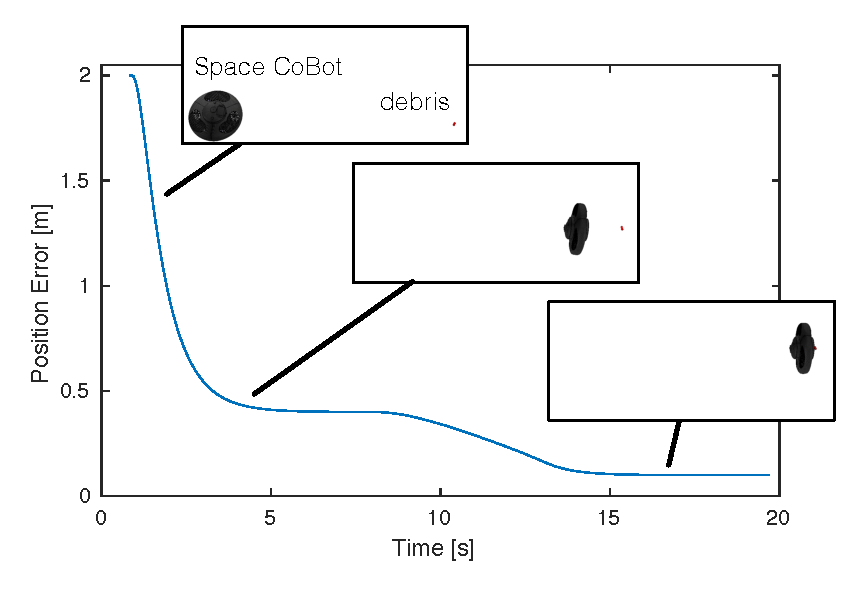
\includegraphics[width=\linewidth]{figs/debris_comp.pdf}
  \caption{Simulation results for debris scavenging: distance from Space
    CoBot to the object position, along the three phases explained in
    the text.}
  \label{fig:debris-results}
\end{figure}

\begin{figure*}
  \centering
  \subfloat[hit with a table]{%
    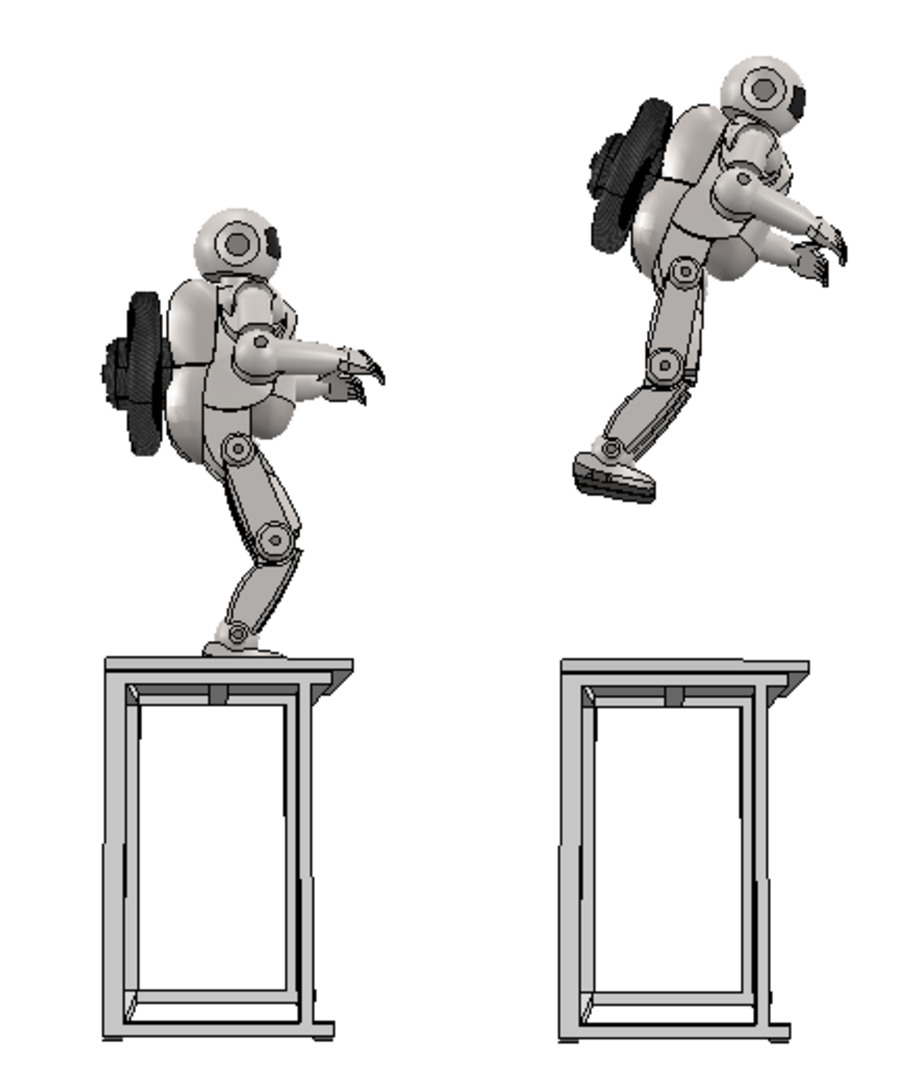
\includegraphics[width=0.3\linewidth]{figs/astri_table.pdf}}
  \qquad
  \subfloat[hit with a wall]{%
    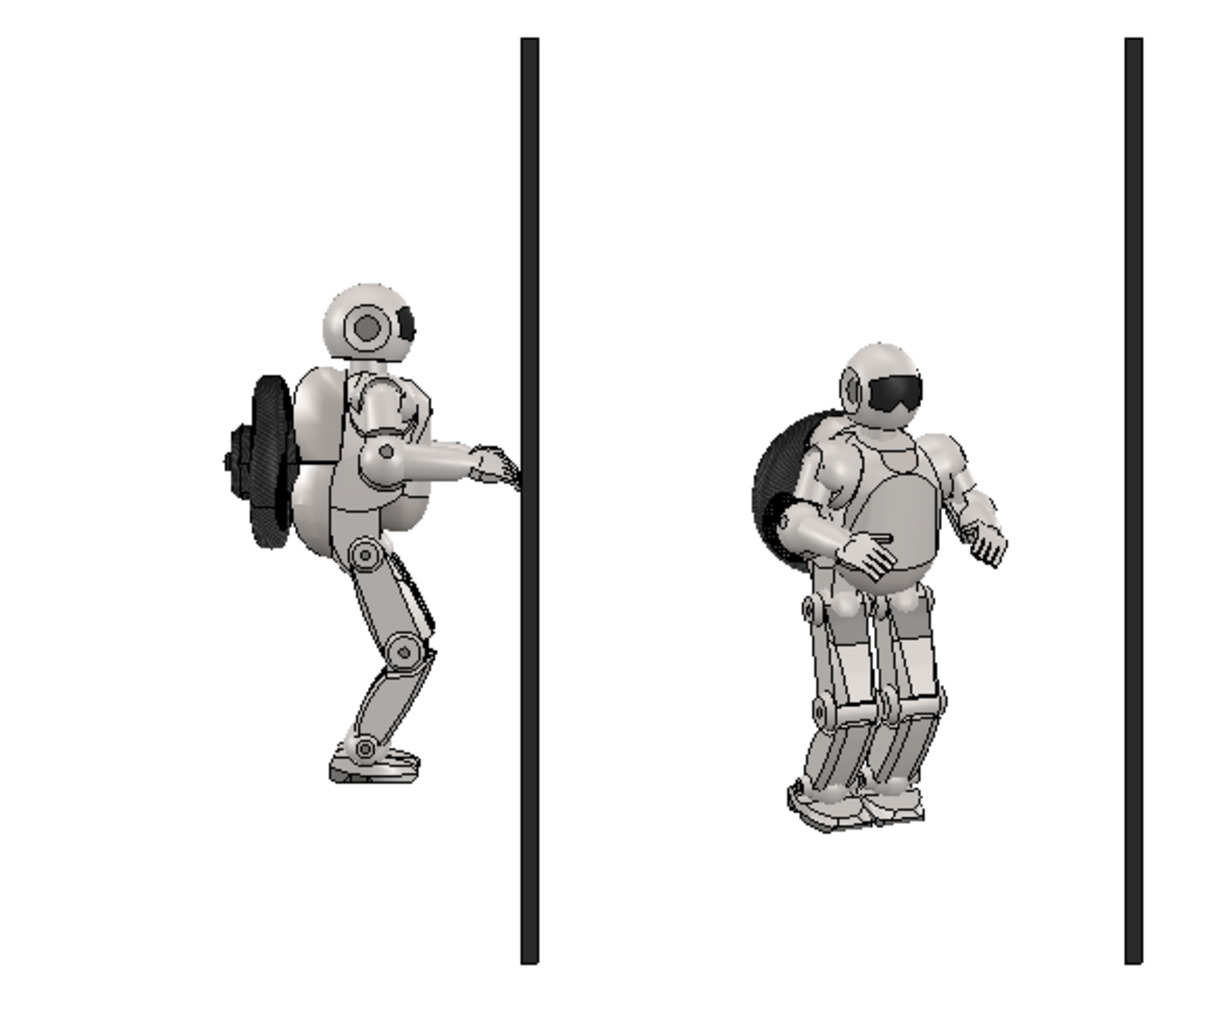
\includegraphics[width=0.3\linewidth]{figs/astri_wall.pdf}}
  \caption{The two simulated situations for the astronaut
    stabilization task.}
  \label{fig:astri_table_wall}
\end{figure*}

In microgravity, it is hard to keep the same position through time, as every little touch 
on indoor surfaces create a linear velocity and angular momentum on the astronauts body.
To overcome such problem, there are steel bars throughout the space station, which one
can grab and stabilize. Although this is a simple solution, there are situations in which 
these cannot be used, either because the user is performing a manual operation or because
these bars are out of range. 

Targeting these situations, we studied the use of a Space CoBot
attached to the back of the astronaut, like a backpack, that actively
uses its propulsion to reduce the astronaut velocity to zero, thus
stopping him from drifting. This is performed by using velocity
feedback only, that is, setting $\bar{v}_d=\bar{\omega}_d=0$ and
disabling the position/attitude feedback with $k_x=k_R=0$. By doing
so, the controller will counteract any non-zero motion of the
astronaut, both translational and rotational, while ignoring its
position.


% As we just want to stop the motion of the astronaut, the Proportional gained was turned off for 
% both experiments.

%On Section \ref{sec:sim-res} we provide the results for both tasks.



\section{Simulation Results}
\label{sec:sim-res}

The realistic simulator V-REP~\cite{vrep13} was used to validate the
approach. Results showing convergence of the controller to
arbitrary setpoints have been previously shown in~\cite{yoda:arxiv16a},
including sensitivity to localization noise and to unmodeled dynamics,
e.g., an heavy load attached to the robot. In this paper we focus on
showing simulations of the debris scavenging and astronaut
stabilization tasks.

Figure~\ref{fig:debris-results} shows a simulation result of the
debris scavenging task. The target object is moving at a constant velocity of
0.03m/s along the $Y$ axis, while Space CoBot goes through the three
phases described above, also indicated in the figure. The distance between
the Space CoBot and the debris is plotted in this figure. Two plateaus
are visible: at $D_1=0.4m$, where Space CoBot matches the debris velocity,
and at $D_2=0.1m$, when we consider the object to be reachable by the robot.

% UPDATE THIS: For the first scene, Figure \ref{fig:debris-results} (a) illustrates the procedure described 
% on Section \ref{sec:debis-scavenging}. Plotted on Figure \ref{fig:debris-results} (b) is the norm of 
% the position error, relative to the object tracked. Note that this error
% does not converge to zero, as it is obtained by the difference between the
% the Center of Mass (CoM) of the space cobot and the CoM of the object and, therefore,
% a zero position error would mean that the object would be inside the robot. 

% On this image we can observe the 2 movement stages refered in  
% Section \ref{sec:debis-scavenging}. First, the robot stabilizes at 0.4 meters
% away of the debree and then it starts to approach the object linearly, until it
% is ready to be caught.

% \begin{figure*}
%   \def\gs{0.3}
%   \centering
%   \subfloat[]{\vbox{%
%       \def\gw{0.2}
%       \hbox{\fbox{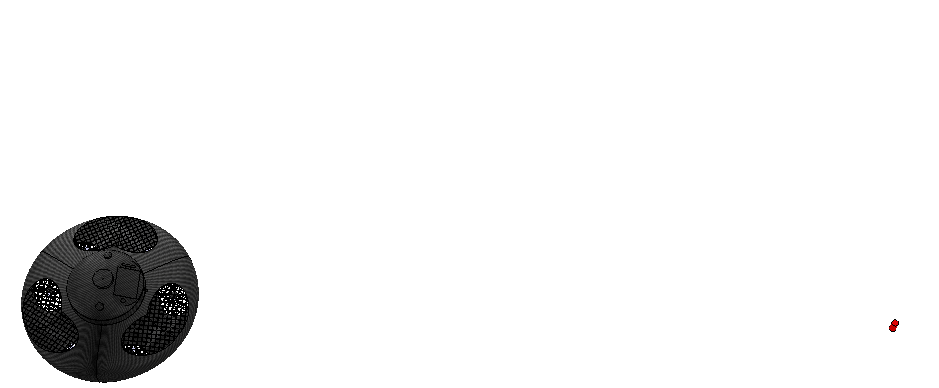
\includegraphics[width=\gw\linewidth]{figs/instace-1.png}}}
%       \hbox{\fbox{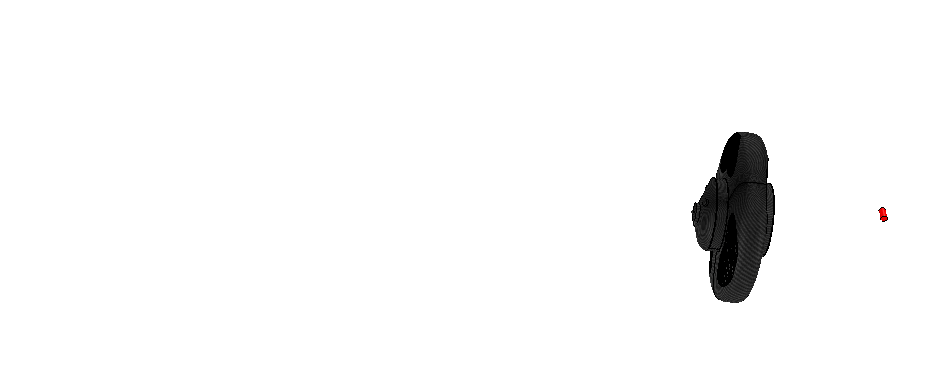
\includegraphics[width=\gw\linewidth]{figs/instace-2.png}}}
%       \hbox{\fbox{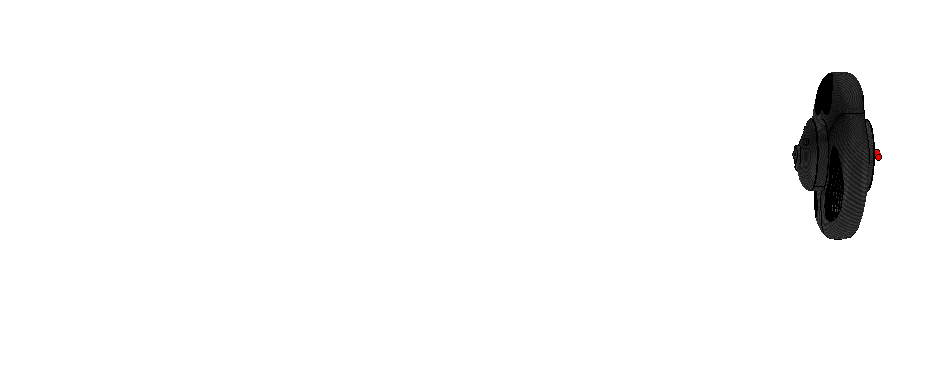
\includegraphics[width=\gw\linewidth]{figs/instace-3.png}}}
%       \hbox{\fbox{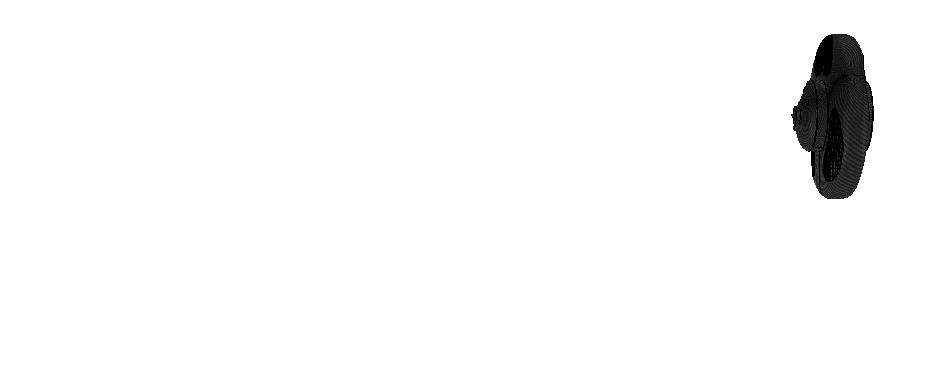
\includegraphics[width=\gw\linewidth]{figs/instace-4.png}}}
%     }}
%   \hfil
%   \subfloat[]{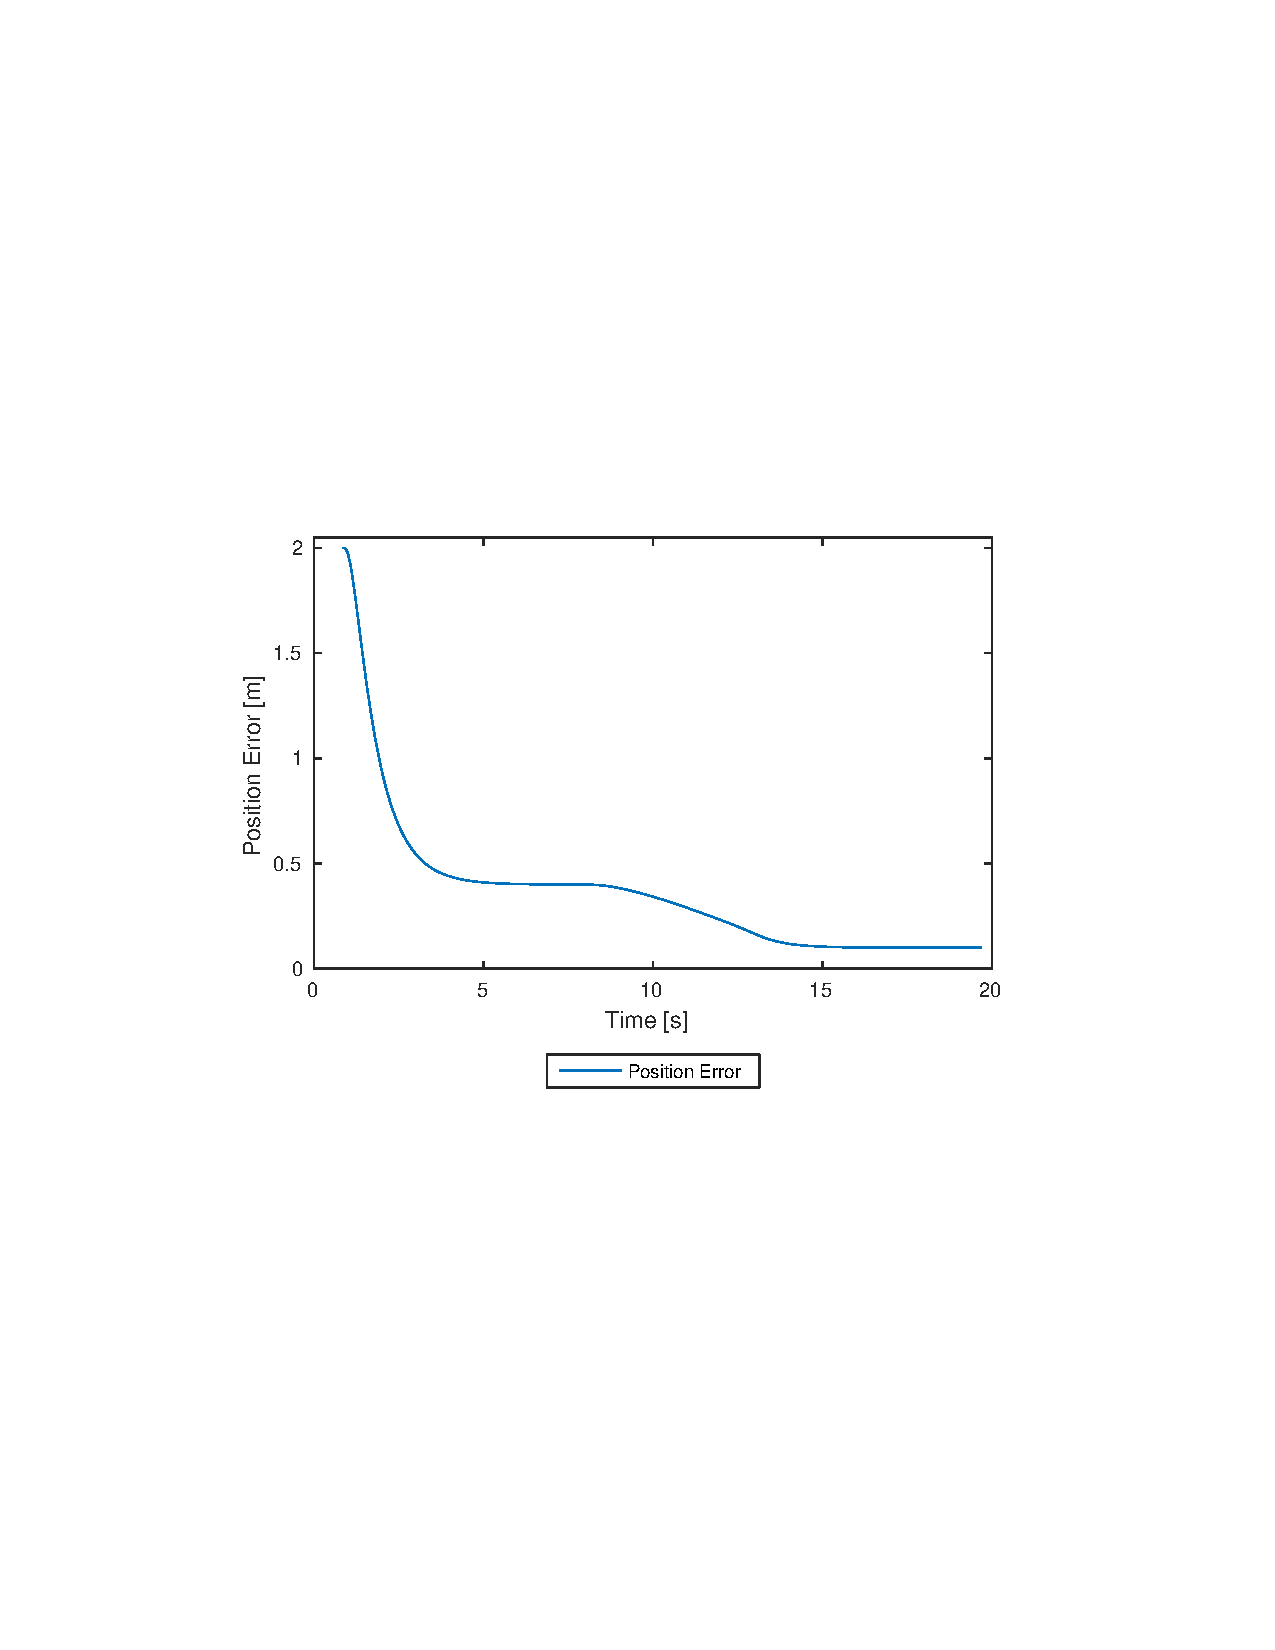
\includegraphics[height=\gs\linewidth, clip=true,
%       trim=4cm 10.3cm 4.5cm 8.8cm]{figs/debree.pdf}}
%   \caption{Debree Scavanging: (a)~trajectory performed by the Space CoBot;
%   to capture the debree; (b)~Norm of the Position Error in respect to the debree.}
%   \label{fig:debris-results}
% \end{figure*}

%, clip=true, trim=3.8cm 9.5cm 4.5cm 8.8cm


% \begin{figure}
% \centering
% \subfloat[]{%
%   \includegraphics[clip,width=0.5\columnwidth]{figs/table.pdf}%
% }
% \subfloat[]{%
%   \includegraphics[clip,width=0.9\columnwidth]{figs/astronaut-table.pdf}%
% }
% \caption{Astronaut Stabilization: (a)~Astronaut jumping on a fixed table;
% (b)~Norm of the velocity error along time, with and without stabilization, on
% the Space CoBot Center of Mass.}
% \label{fig:astronaut-table}
% \end{figure}

To simulate the astronaut stabilization task, we used the Astri
humanoid model, bundled with V-REP, to emulate the body dynamics of an
astronaut. Its total mass is 73Kg (12 times heavier than Space
CoBot). We tested two situations, illustrated in
Figure~\ref{fig:astri_table_wall}: in (a)~the astronaut stretches his
legs and hits the top of a table, while in (b)~the astronaut stretches his
arms and hits a vertical wall. In both cases, the hit provokes a
reaction momentum impelling the astronaut on the opposite direction to
the hit.

% The test is composed by two two experiments: on the first, we immobilize an astronaut
% --- represented in the simulation by the Asti robot model, with a
% total mass of 73kg, 12 times more than Space CoBot --- while
% it does a small jump; on the second we immobilize the individual when he pushes himself against 
% a wall.
 
% On the second scene, Figure \ref{fig:astronaut-table} (a) illustrates the jumping scene,
% while Figure \ref{fig:astronaut-table} (b), shows the results of jumping
% with and without active stabilization, through the plots of the norm for
% the velocity error.

For each one of these situations we compared the trajectories of Space
CoBot, always attached to the astronaut, with and without the
controller. Plots of the translational velocity norm of the robot CoM
are shown in Figure~\ref{fig:table-wall-plot}. It is visible in both
cases that the controller successfully stabilizes motion in about 4
seconds. The oscillatory behavior when the controller is disabled
corresponds to the velocity, with respect to the inertial frame, of
the robot CoM ``orbiting'' the resultant CoM of astronaut+robot, while
it drifts away from the contact point.

\begin{figure*}
  \centering
  \subfloat[hit with a table]{%
    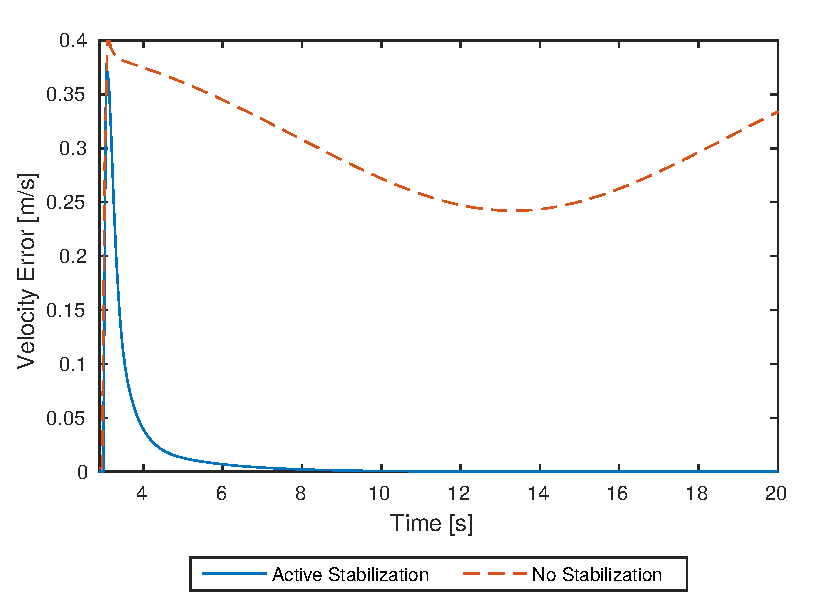
\includegraphics[width=0.47\linewidth]{figs/plot_table.pdf}} \qquad
  \subfloat[hit with a wall]{%
    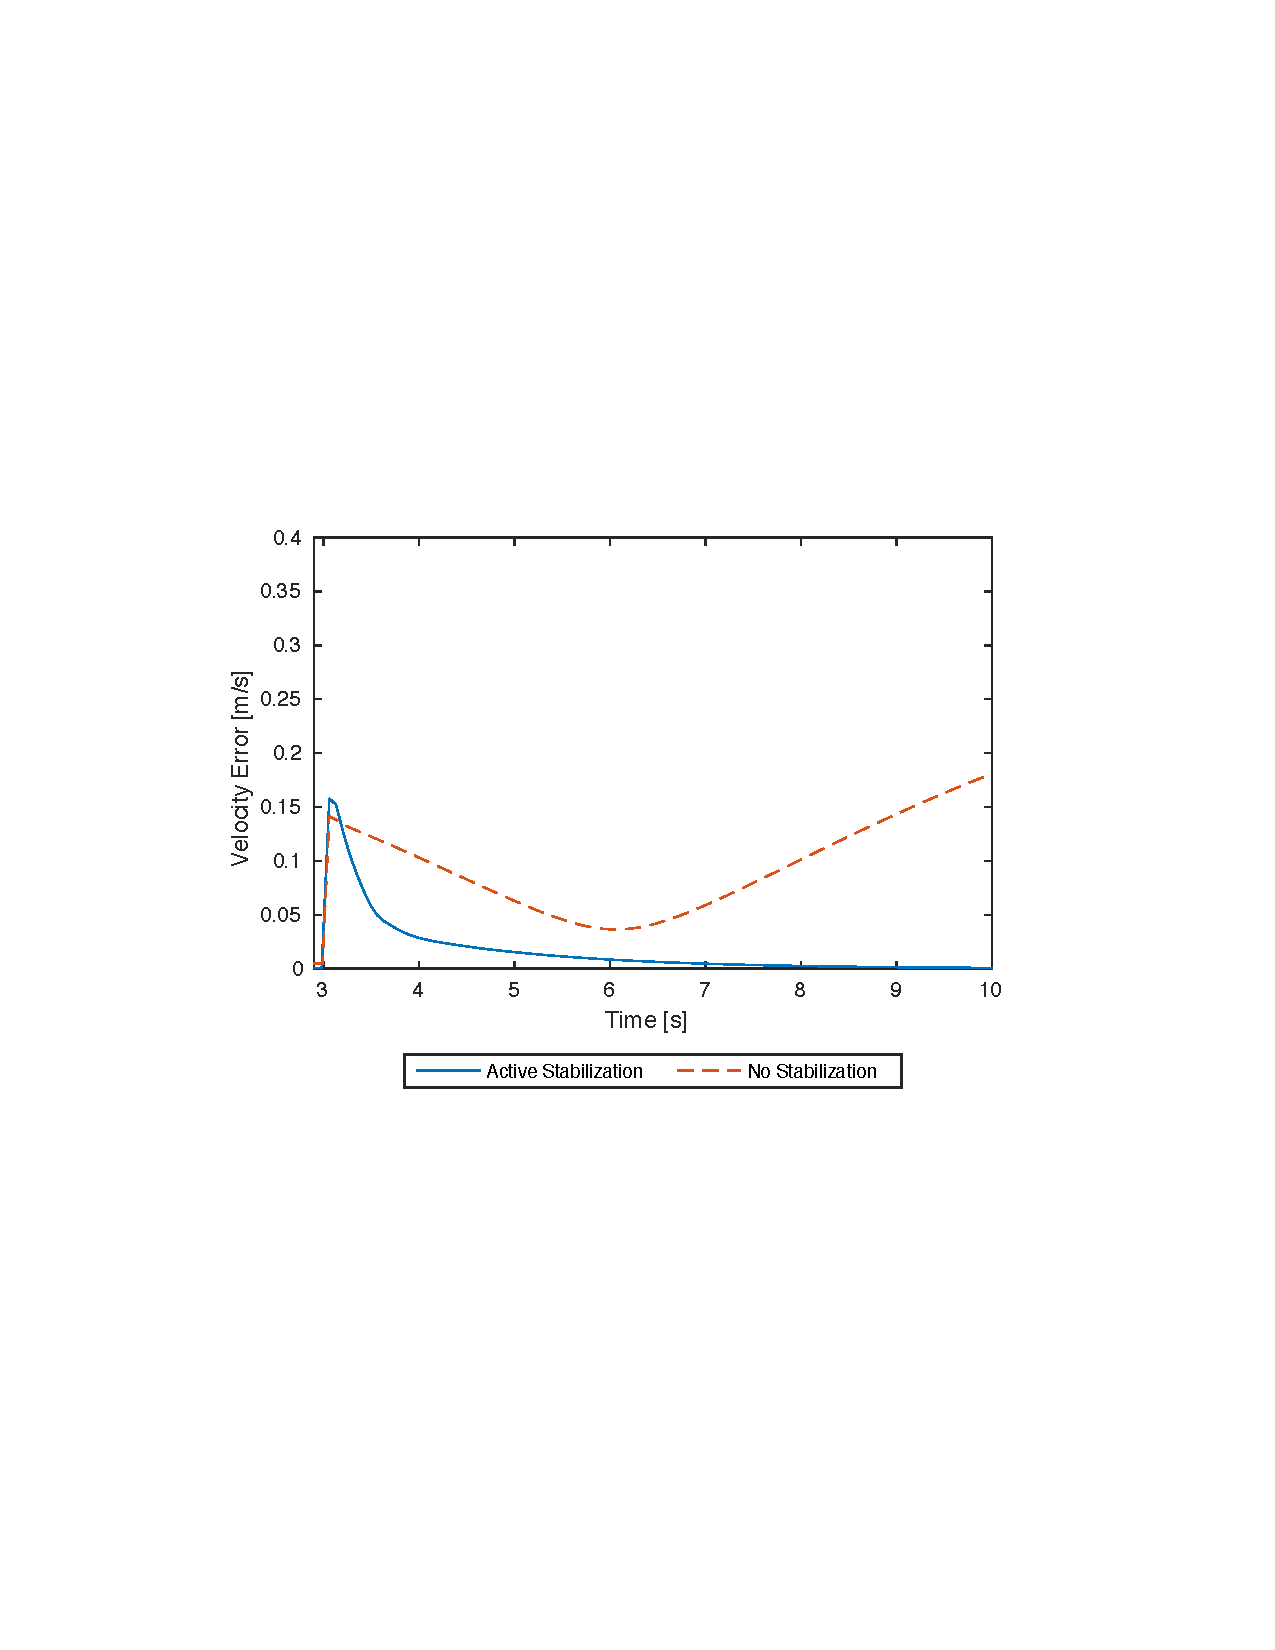
\includegraphics[width=0.47\linewidth]{figs/plot_wall.pdf}}
  \caption{Norm of the linear velocity of Space CoBot, with and
    without motion stabilization, for the two situations described in
    the text.}
  \label{fig:table-wall-plot}
\end{figure*}

% When activated, the Space CoBot can successfully stabilize an astronaut in about
% 3 seconds, even though it has 12 times less the mass of astronaut model.
% Note that the velocity norm error presented is expressed for the robot CoM, and for the 
% CoM of the joint masses. Therefore, as the astronaut spins, the velocity without
% stabilization oscillates due to the momentum imposed by the force of the jumping movement.

All of the simulations discussed in this section were compiled into a
video available here: \\
\centerline{\url{https://youtu.be/TQqRAMBv3-M}}

\section{Conclusions and Future Work}
\label{sec:concl-future-work}

This paper presented both the design and the application of Space
CoBot for assistive tasks to astronauts, to operate inside
orbiting space stations. It is based on a hexarotor design with a
fully holonomic kinematics. A convergent motion controller was presented, which
was then used to explore two applications. The first one is
scavenging of free flying debris, while the second one is motion
stabilization of astronauts. These application were implemented and
evaluated with a realistic robotics simulator.

Future work will proceed in two directions: on the one hand, to build
a real prototype to validate approach (partially on Earth, and in full
on, e.g., parabolic flight tests), and on the other, to address basic
functionalities such as vision-based navigation and human-robot
interaction.


%% The file named.bst is a bibliography style file for BibTeX 0.99c
\bibliographystyle{named}
\bibliography{biblio}

\end{document}
